\documentclass[11pt]{exam}
\usepackage[empty]{fullpage}
\usepackage{amsmath}
\usepackage{tikz,pgfplots}
\usepackage{soul}
\usepackage{pdfpages}

\newcommand{\ds}{\displaystyle}


\begin{document}
\graphicspath{{/home/brian/Dropbox/HSC/Spring13/Math121/}}

\subsection*{Statistical Methods - Math 222 \hfill Final Exam Review Problems}

\textit{The final exam will be on \textbf{Thursday, April 30 at 2:00pm}. The following problems are similar to ones you might see on the final exam.}


\begin{questions}

\question The regression model below is based on the listed CarMax.com ``no-haggle prices" and mileage of a random sample of 33 used Honda Civics on sale in the Richmond area.

{\small
\begin{verbatim}
## Call:
## lm(formula = Price ~ Mileage, data = civicData)
## 
## Residuals:
##     Min      1Q  Median      3Q     Max 
## -2722.5  -649.8   -77.2   516.5  4269.1 
## 
## Coefficients:
##               Estimate Std. Error t value Pr(>|t|)    
## (Intercept)  18000.41     493.11   36.50  < 2e-16 ***
## Mileage      -0.08105    0.01204   -6.73 1.57e-07 ***
## ---
## Signif. codes:  0 '***' 0.001 '**' 0.01 '*' 0.05 '.' 0.1 ' ' 1
## 
## Residual standard error: 1269 on 31 degrees of freedom
## Multiple R-squared:  0.5937, Adjusted R-squared:  0.5806 
## F-statistic: 45.29 on 1 and 31 DF,  p-value: 1.567e-07
\end{verbatim}
}
\begin{parts}
\part What is the equation for the least squares regression line?
\vfill

\part How much would a Civic with 80,000 miles cost, on average? 
\vfill

\part A 90\% prediction interval for the price of a Civic with 80,000 miles is: \$9,160 to  \$13,870. Explain how this prediction interval is different than a confidence interval.  
\vfill

\part Make a 95\% confidence interval for the \underline{slope} of the regression line, and clearly describe the parameter of interest that we are confident will be in this interval.  Hint: The right critical $t$-value for this confidence interval is $t^* = 2.0395$.
\vfill


\end{parts}

\newpage

\question Here is the scatterplot and trend line showing the relationship between Civic prices and mileage.  What would you say is the biggest source of concern about our linear regression model?   
\begin{flushright}
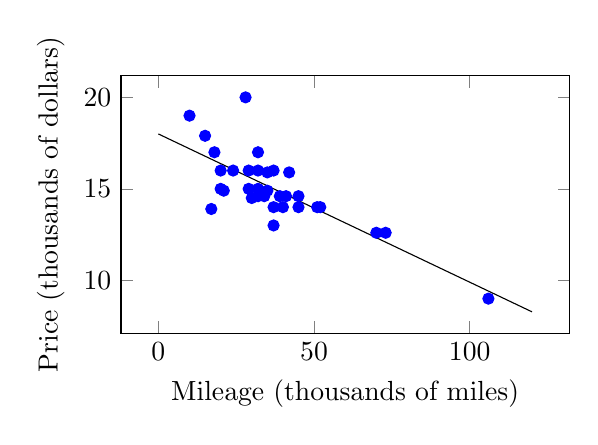
\begin{tikzpicture}
    \begin{axis}[
        xlabel=Mileage (thousands of miles),
        ylabel=Price ({thousands of dollars}),
        width = 0.6\textwidth,
        height = 0.4\textwidth,
        yticklabel style={
            /pgf/number format/fixed,
            /pgf/number format/precision=5
	    },
		scaled y ticks=false,
	    ylabel near ticks
        ]
    \addplot[only marks,mark=*,blue] plot coordinates {
(106, 9)
(37, 13)
(37, 16)
(40, 14)
(32, 14.6)
(10, 19)
(24, 16)
(32, 16)
(28, 20)
(34, 14.6)
(41, 14.6)
(45, 14.6)
(52, 14)
(32, 17)
(20, 15)
(39, 14.6)
(20, 16)
(32, 15)
(51, 14)
(73, 12.6)
(70, 12.6)
(29, 15)
(29, 16)
(37, 14)
(45, 14)
(35, 15.9)
(42, 15.9)
(17, 13.9)
(21, 14.9)
(15, 17.9)
(30, 14.5)
(35, 14.9)
(18, 17)
    };
\addplot[domain=0:120] {-0.081*x + 18.0};
\end{axis}
\end{tikzpicture}
\end{flushright}

\bigskip


\question The following data shows the amount of rainfall produced (in acre-feet) on 26 random days when an airplane sprayed clouds with a silver-iodide solution in an experiment on cloud seeding. 
{\footnotesize
\begin{verbatim}
   4.1,    7.7,   17.5,   31.4,   32.7,   40.6,   92.4,  115.3,  118.3,  119.0,  129.6,  198.6,  200.7, 
 242.5,  255.0,  274.7,  274.7,  302.8,  334.1,  430.0,  489.1,  703.4,  978.0, 1656.0, 1697.8, 2745.6, 
\end{verbatim}
}

\begin{parts}
\part Make a histogram for this data with bins that are 500 acre-feet wide. 
\vfill
\vfill
\vfill

\part Explain why it might be a good idea to apply a log-transform before applying t-distribution techniques to this data. 
\vfill

\part Suppose that the data is approximately normally distributed after a log-transform. A 95\% confidence interval for the mean of the log-transformed data is 4.49 to 5.78.  What does this tell us about the \underline{median} rainfall on similar days with cloud seeding?  
\vfill
\end{parts}


\newpage
\question The sample correlation between the price of a used Civic and its mileage is $-0.77$.  Unlike slope, the summary command in R does not provide a standard error for the correlation.  Below is R code and output for a bootstrap distribution for the correlation coefficient.  

{\small
\begin{verbatim}
boot.dist = c()
for (i in 1:200) {
  boot.sample = civicData[sample(33,replace=T),]
  boot.stat = cor(boot.sample$Mileage,boot.sample$Price)
  boot.dist = c(boot.dist,boot.stat)
}
sort(boot.dist)

##   [1] -0.9420432 -0.9406652 -0.9384148 -0.9300384 -0.9074382 -0.9032975
##   [7] -0.9020444 -0.9013100 -0.8865266 -0.8859943 -0.8851801 -0.8842967
##  [13] -0.8841325 -0.8790962 -0.8747007 -0.8744395 -0.8738456 -0.8714636
##  [19] -0.8713282 -0.8698345 -0.8690512 -0.8676675 -0.8676001 -0.8670668
##  [25] -0.8670346 -0.8642180 -0.8621218 -0.8616683 -0.8613130 -0.8610971
##  [31] -0.8596772 -0.8580612 -0.8572514 -0.8563220 -0.8560142 -0.8559836
##  [37] -0.8532574 -0.8513093 -0.8502798 -0.8480401 -0.8479187 -0.8470201
##  [43] -0.8451717 -0.8422841 -0.8403520 -0.8362966 -0.8359552 -0.8349236
##  [49] -0.8344944 -0.8335796 -0.8304102 -0.8296235 -0.8285763 -0.8245773
##  [55] -0.8245378 -0.8245300 -0.8244075 -0.8231082 -0.8208700 -0.8186366
##  [61] -0.8172532 -0.8171862 -0.8171750 -0.8165555 -0.8148891 -0.8148768
##  [67] -0.8104966 -0.8090642 -0.8083473 -0.8073777 -0.8010170 -0.8008010
##  [73] -0.8001316 -0.7981386 -0.7967867 -0.7967547 -0.7947311 -0.7924981
##  [79] -0.7918131 -0.7911701 -0.7910251 -0.7907357 -0.7875289 -0.7839404
##  [85] -0.7838220 -0.7825485 -0.7814483 -0.7813557 -0.7810032 -0.7798871
##  [91] -0.7780595 -0.7780324 -0.7685441 -0.7683411 -0.7681656 -0.7676848
##  [97] -0.7666294 -0.7662148 -0.7659370 -0.7645721 -0.7639991 -0.7619817
## [103] -0.7588827 -0.7583176 -0.7582218 -0.7560310 -0.7560066 -0.7552945
## [109] -0.7542569 -0.7539496 -0.7532599 -0.7531970 -0.7522636 -0.7494382
## [115] -0.7447879 -0.7421428 -0.7375672 -0.7357633 -0.7338413 -0.7324574
## [121] -0.7315154 -0.7282993 -0.7281583 -0.7256986 -0.7253234 -0.7195348
## [127] -0.7138319 -0.7124563 -0.7117652 -0.7110178 -0.7096631 -0.7089917
## [133] -0.7079075 -0.7021989 -0.6995537 -0.6992297 -0.6965921 -0.6927159
## [139] -0.6898840 -0.6856175 -0.6847421 -0.6844857 -0.6844375 -0.6825583
## [145] -0.6813276 -0.6793608 -0.6734295 -0.6651888 -0.6629154 -0.6625288
## [151] -0.6610533 -0.6603110 -0.6579832 -0.6516430 -0.6491577 -0.6425978
## [157] -0.6422529 -0.6355755 -0.6316805 -0.6301139 -0.6245669 -0.6212388
## [163] -0.6194756 -0.6191732 -0.6191051 -0.6156924 -0.6125584 -0.6097496
## [169] -0.6083101 -0.5940321 -0.5931356 -0.5885409 -0.5844738 -0.5798155
## [175] -0.5771780 -0.5684650 -0.5679013 -0.5644295 -0.5567876 -0.5521994
## [181] -0.5505885 -0.5406679 -0.5389025 -0.5373632 -0.5365104 -0.5219112
## [187] -0.5186793 -0.5149354 -0.5113523 -0.5066999 -0.5042188 -0.4975819
## [193] -0.4963595 -0.4228281 -0.4060593 -0.3921223 -0.3757002 -0.3701165
## [199] -0.3382373 -0.2841541
\end{verbatim}
}

Use this information to find a 90\% bootstrap confidence interval for the (population) correlation between mileage and price of used Honda Civics.  
\vfill

\newpage
\question The following logistic regression model is based on a sample of 200 patients admitted to the Intensive Care Unit at one hospital.  The variables include the \verb|Age| of the patient, systolic blood pressure \verb|SysBP| (in mm of Hg) when admitted, and \verb|Survive| which is a binary indicator variable that is 1 if the patient lived to be discharged and 0 if they died. 

\begin{verbatim}
## Call:
## glm(formula = Survive ~ Age + SysBP, family = "binomial", data = icu)
## 
## Coefficients:
##              Estimate Std. Error z value Pr(>|z|)   
## (Intercept)  0.962471   1.000272   0.962  0.33594   
## Age         -0.028407   0.010774  -2.637  0.00838 **
## SysBP        0.016831   0.005859   2.873  0.00407 **
\end{verbatim}

\begin{parts}
\part What is the formula for the logistic regression model? 
\vfill

\part The first person in the data set was an 87 year old man with a systolic blood pressure of 80.  What does the logistic regression model above predict for the probability that this man survived?
\vfill


\part How much do the odds of survival go down for every year older a patient is?  
\vfill  


\end{parts}

\question What is the definition of a p-value? 
\vspace*{1in}

\question A group of student volunteers at one University participated in a blind taste test comparing Coke vs. Pepsi. In the test, 29 students preferred the taste of Coke, while 42 preferred Pepsi. 
\begin{parts}
\part What command in R could you use to make a confidence interval for the percent of students who prefer Coke? 
\vfill

\part If you start with a uniform prior distribution, then what is the posterior distribution for the proportion of students who prefer Coke?
\vfill

\part What R command(s) could you use to get a 95\%-credible interval for the proportion of students who prefer Coke in a blind taste test?
\vfill
\end{parts}

\newpage
\question A sociologist is interested in whether journals like \textit{Nature} or \textit{Science} tend to use different terminologies compared to more technical journals. For instance, the word `network' can be hypothesized to appear more frequently in technical papers. The researcher takes a random sample of 120 authors who have published at least one article in \textit{Nature} and one article in \textit{Cell}, and then randomly selects one article in each of these two journals from each author. Then, for each article, the researcher finds the number of occurrences of `network', and divides by the total number of words in the article. Is this data better suited to analysis using an independent samples t-test, or a matched pairs t-test, and why?
\vfill


\question A study looked at a random sample of 12 counties in Iowa (stratified by the size of the county: small, medium, large) and counted the number of methamphetamine labs in each county. The researchers wanted to determine whether county size is a significant factor in the determining the number of labs. Use the ANOVA table below to answer the following questions. 

\begin{center}
\renewcommand{\arraystretch}{2.0}
\begin{tabular}{|l|c|c|c|c|}
\hline
Source & ~~~~ DF ~~~~ & SS & MS & F \\ \hline
Model & ~ & 37.51 & \hspace*{1.1in} & \hspace*{1.1in} \\ \hline 
Error & ~  & \hspace*{1.1in} & ~ & ~ \\ \hline
Total & ~ & 70.60 & ~ & ~ \\ \hline
\end{tabular}
\end{center}
\begin{parts}
\part Fill in the missing values in the table. 
\vfill

\part One of the assumptions of ANOVA is that each group has the same variance.  If this is true, then what number is the best guess for the standard deviation of the number of meth labs per small county?  
\vfill

\part What R command would give the p-value for an ANOVA F-test with this data? 
\vfill

\part Describe the hypotheses tested by the F-test. 
\vfill
\end{parts}



\newpage

\question Is country air better to breathe than city air? One way to address this question is by measuring how quickly a person's lungs clear out unhealthy particles.  Researchers in 1973 found seven pairs of identical twins, where one twin lived in the country and the other lived in a city.  They asked each twin to inhale an aerosol of radioactive Teflon particles and then measured the percentage of the radioactivity remaining after one hour.  The results are in the following table:

\begin{center}
\begin{tabular}{l|ccccccc|cc}
Twin Pair & A & B & C & D & E & F & G & $\bar{x}$ & $s$ \\ \hline
Rural Environment & 10.1 & 51.8 & 33.5 & 32.8 & 69.0 & 38.8 & 54.6 & 41.5 & 19.0 \\
Urban Environment & 28.1 & 36.2 & 40.7 & 38.8 & 71.0 & 47.0 & 57.0 & 45.5 & 14.4 \\ \hline
Difference & 18 & -15.6 & 7.2 & 6 & 2 & 8.2 & 2.4 & 4.0 & 10.2 \\
\end{tabular}
\end{center}

\begin{parts}

\part Was this a randomized controlled experiment?  Why or why not?  
\vfill

\part By studying identical twins, the researchers have controlled for many possible lurking variables, including age, race, gender, and genetics.  Describe one lurking variable that the researchers did not control for.  
\vfill 


\part Notice that the numbers are higher for the urban twin in all but one pair.  If we assume that the sign of the difference for each pair is just random (with even odds), then what is the probability of getting a result at least as extreme as what we got?  \textit{It is okay to write your answer using R code.}
\vfill

\end{parts}

\question The 2008 General Social Survey asked a sample of adult American whether they consider their life to be exciting, routine, or dull.  The results are displayed by gender in the two-way table below.  
\begin{center}
\begin{tabular}{l|cc|c}
~ & Male & Female & Total \\ \hline
Exciting & 300 & 347 & 647 \\
Routine & 284 & 342 & 626 \\
Dull & 21 & 43 & 64 \\
Other & 5 & 7 & 12 \\ \hline
Total & 610 & 739 & 1349  
\end{tabular}
\end{center}
\begin{parts}
\part What are the variables in the two-way table above?  
\vfill

\part What are the correct null and alternative hypotheses for a $\chi^2$-test of association?
\vfill

\part The two-way table has $\chi^2 = 4.39$ which corresponds to a p-value of 22.2\%.  What does that mean?  
\vfill

%\part Collapse the response variable into just two categories: exciting and not. Then conduct a test on the resulting 2-by-2 table.  
%\vfill

%\part What is the odds ratio for comparing the odds that male respondents find their life exciting versus female respondents?  
%\vfill


%\part Use logistic regression (with the collapsed 2-by-2 table) to make a 95\% confidence interval for the odds ratio.  Explain your conclusions.  
%\vfill

\end{parts}


\newpage
\question The herbal supplement Garcinia Cambogia is advocated by Dr. Mehmet Oz (a celebrity doctor) as an effective weight loss aid. A 1998 study of 135 people found that it was no more effective than a placebo. Here is a summary of the results from that study. 

\fbox{
    \begin{minipage}{\textwidth}
        \small
        A total of 135 subjects were randomized to either active hydroxycitric acid [The active ingredient in G. Cambogia] ($n=66$) or placebo ($n=69$); 42 (64\%) in the active hydroxycitric acid group and 42 (61\%) in the placebo group completed 12 weeks of treatment. Patients in both groups lost a significant amount of weight during the 12-week treatment period; however, between-group weight loss differences were not statistically significant (mean [SD], 3.2 [3.3] kg vs 4.1 [3.9] kg; $P=0.14$).
    \end{minipage}
}
Here is a summary of the results of the study.  
\begin{center}
    \begin{tabular}{l|ccc}
        \hline
        Group & $N$ & $\bar{x}$ & $s$ \\ \hline
Treatment & 42  & 4.1       & 3.9 \\
  Control & 42  & 3.2       & 3.3 \\ \hline
    \end{tabular}
\end{center}

\begin{parts}
\part This is an example of a randomized controlled experiment.  Why is it important to use a randomized controlled experiment in this situation instead of an observational study? 
\vfill

\part What are the explanatory and response variables?  
\vfill

\part When they say that ``patients in both groups lost a significant amount of weight", what do they mean?  What statistical test or tests did they use? (You don't need to compute anything, just name the test and state the relevant hypotheses.)
\vfill
\vfill


\part Where did the $P=0.14$ number come from? What R command could they use to get that number? (You don't need to calculate anything.)
\vfill
\vfill

\part According to the researchers, the effect of Garcinia Cambogia is not statistically significant because the $p$-value was 0.14. Which of the following best describes what this means. 
\begin{choices}
\part The placebo is just as effective as Garcinia Cambogia.  
\part There might be one or more lurking variables that explain the difference.
\part This proves that Garcinia Cambogia doesn't help people lose weight.
\part The observed difference might have been a fluke.   
\end{choices}
\bigskip


\part Suppose we wanted to do a follow-up study with 200 people in each group.  Let's assume that the true effect size of G. Cambogia is 0.5 extra kg weight loss over the placebo, on average and the true standard deviation in weight loss for both groups is $\sigma = 4$ kg. Estimate the power of a two-sample test to detect this difference using the normal distribution.  Write your answer using R code.  
\vfill


\end{parts}
\end{questions}
\end{document}
